% !TeX root = ../main.tex
\chapter{System Design and Architecture}
\label{ch:architecture}

This chapter presents the system architecture decisions that enabled the HPC Sorting Serious Game to be feasible, maintainable, and pedagogically interpretable. It focuses on architectural structure and rationale rather than exhaustive implementation listings. Detailed implementation is provided in Chapter~\ref{ch:implementation}, and educational/operational effectiveness is evaluated in Chapter~\ref{ch:results}.

%-----------------------------------------------------------------------
\section{Architectural Overview}
\label{sec:architectural-overview}

The architecture is organized to support two complementary goals:
\begin{itemize}
    \item \textbf{Pedagogical clarity}: game mechanics must remain interpretable as OpenMP-inspired shared-memory collaboration.
    \item \textbf{Technical robustness}: multiplayer synchronization must remain consistent across browser clients under variable latency.
\end{itemize}

%-----------------------------------------------------------------------
\subsection{Design Principles}
\label{subsec:design-principles}

The architecture is guided by the following principles:
\begin{enumerate}
    \item \textbf{Component modularity}: cards, buffers, and managers are separated so mechanics can evolve without rewriting the whole system.
    \item \textbf{Separation of concerns}: UI, game rules, and synchronization logic are isolated to reduce coupling during iterative experiments.
    \item \textbf{Host-authoritative conflict handling}: one authority resolves contested actions to prevent divergent multiplayer states.
    \item \textbf{Observable synchronization}: architecture includes explicit state transitions that can be logged and inspected during debugging.
    \item \textbf{Web-first constraints}: transport, update cadence, and payload design prioritize browser compatibility over engine-native networking assumptions.
\end{enumerate}

%-----------------------------------------------------------------------
\subsection{System Layers}
\label{subsec:system-layers}

\begin{description}
    \item[Presentation Layer] Renders cards, buffers, indicators, and interaction feedback.
    \item[Game Logic Layer] Validates sorting actions, completion conditions, and per-mode rules.
    \item[Synchronization Layer] Coordinates shared/private state propagation, ordering, and conflict resolution.
    \item[Transport/Relay Layer] Handles browser-compatible signaling and event relay via HTTP/SSE.
\end{description}

These layers decouple pedagogical behavior from transport mechanics, which was essential when adapting multiplayer behavior for browser export.

%-----------------------------------------------------------------------
\section{Scene and Interaction Architecture}
\label{sec:scene-structure}

The scene model is intentionally concise: a menu/lobby entry path and two gameplay contexts (single-player baseline and multiplayer OpenMP-style collaboration). The scene split supports direct comparison between sequential and collaborative execution while reusing core card and validation logic.
% TODO: [Artifact] Consolidated scene-transition/state diagram.
% TODO: [Purpose] Explain lifecycle transitions and their pedagogical meaning.
% TODO: [Source Inputs] scene_manager.gd; scenes/MainMenuScene/menu_scene.tscn; scenes/Multiplayer/Lobby/multiplayer_lobby.gd.
% TODO: [Placement] In this section, immediately after the "Architectural Intent" bullets.
% TODO: [Done Criteria] Include paths MainMenu -> SinglePlayer, MainMenu -> Lobby -> MultiplayerGame, and Gameplay -> Completion; each arrow must state trigger and learning implication.
% TODO: [Cross-refs] Chapter~\ref{ch:results}, Section~\ref{subsec:use-cases}.

\paragraph*{Architectural Intent:}
\begin{itemize}
    \item Single-player provides the sequential baseline for speedup interpretation.
    \item Multiplayer preserves shared container semantics while enforcing private buffer visibility.
    \item Lobby separates session orchestration from gameplay state transitions.
\end{itemize}

This scene structure keeps learning signals (who can see what, who can move what, when state is final) explicit for both users and evaluators.

%-----------------------------------------------------------------------
\subsection{Scene Lifecycle and Transition Logic}
\label{subsec:scene-lifecycle}

Scene changes are managed through a central scene manager to avoid ad-hoc transitions across gameplay scripts. This keeps navigation behavior deterministic and makes it easier to relate transitions to teaching intent (e.g., sequential baseline first, then collaborative mode).

%-----------------------------------------------------------------------
\subsection{Event-Driven Coordination}
\label{subsec:event-driven-architecture}

The architecture is event-driven at component boundaries. Local game objects communicate via Godot signals, while multiplayer state changes are propagated through authority-managed synchronization paths. This split allows UI responsiveness without directly coupling UI events to transport internals.
% TODO: [Artifact] Signal-flow map for one local interaction path and one multiplayer path.
% TODO: [Purpose] Show emitter/listener relationships and where authority checks occur.
% TODO: [Source Inputs] scenes/CardScene/scripts/card_manager.gd; scenes/Multiplayer/connection_manager.gd; scenes/Multiplayer/Lobby/multiplayer_lobby.gd.
% TODO: [Placement] End of this subsection, before Section~\ref{sec:core-components}.
% TODO: [Done Criteria] Include at least one local signal path and one connection/lobby event path with explicit event names.
% TODO: [Cross-refs] Section~\ref{subsec:connection-management}; Chapter~\ref{ch:implementation}, Section~\ref{subsec:lobby-system}.

%-----------------------------------------------------------------------
\section{Core Component Roles}
\label{sec:core-components}

Rather than duplicating full class implementations, this section summarizes architecture-critical component responsibilities.
% TODO: [Artifact] Compact UML/component-inheritance diagram.
% TODO: [Purpose] Document reusability-oriented class boundaries and extension points.
% TODO: [Source Inputs] scenes/CardScene/scripts/card_manager.gd; scenes/Multiplayer/MultiplayerGame/multiplayer_card_manager.gd.
% TODO: [Placement] After the Multiplayer Card Manager paragraph.
% TODO: [Done Criteria] Show CardManager -> MultiplayerCardManager inheritance and manager responsibility split.
% TODO: [Cross-refs] Chapter~\ref{ch:implementation}, Section~\ref{sec:impl-core-components}.

\paragraph*{Card Component (Interaction Unit):}
\label{subsec:card-component}
\begin{itemize}
    \item Encapsulates value identity, interaction state, and visual feedback states.
    \item Emits events consumed by manager-level logic rather than mutating global state directly.
\end{itemize}

\paragraph*{Card Manager (Rule and State Coordinator):}
\label{subsec:card-manager}
\begin{itemize}
    \item Owns sorting validity checks and authoritative placement updates.
    \item Serves as the integration boundary between UI interaction and synchronization rules.
    \item Was designed for reusability: shared logic lives in \texttt{card\_manager.gd} so mode-specific behavior can be layered instead of duplicated.
\end{itemize}

\paragraph*{Multiplayer Card Manager (Authority Extension):}
\label{subsec:multiplayer-card-manager}
\begin{itemize}
    \item Explicitly extends \texttt{card\_manager.gd} as \texttt{multiplayer\_card\_manager.gd}, adding host-authoritative synchronization and reconciliation behavior while reusing baseline card/rule logic.
    \item Enforces shared/private visibility semantics across peers.
\end{itemize}

%-----------------------------------------------------------------------
\section{Multiplayer Architecture}
\label{sec:multiplayer-architecture}

%-----------------------------------------------------------------------
\subsection{Network Topology}
\label{subsec:network-topology}

The implemented multiplayer topology uses browser-compatible relay patterns for session events and state updates. This avoids assumptions that are unstable in browser-exported runtime contexts.
% TODO: [Artifact] Deployment/context diagram with authority boundaries.
% TODO: [Purpose] Distinguish in-process signal communication from inter-client relay communication.
% TODO: [Source Inputs] figures/diagrams/http-sse-architecture.png; scenes/Multiplayer/connection_manager.gd; scenes/Multiplayer/GDSyncWebPatch/local_server_signaling.gd.
% TODO: [Placement] Near Figure~\ref{fig:http-sse-architecture}, as a companion context figure.
% TODO: [Done Criteria] Show browser clients, signaling/relay server, host authority decision point, and shared/private state propagation boundary.
% TODO: [Cross-refs] Chapter~\ref{ch:problems}, Section~\ref{subsec:web-patch-case-study}.

\begin{figure}[htbp]
    \centering
    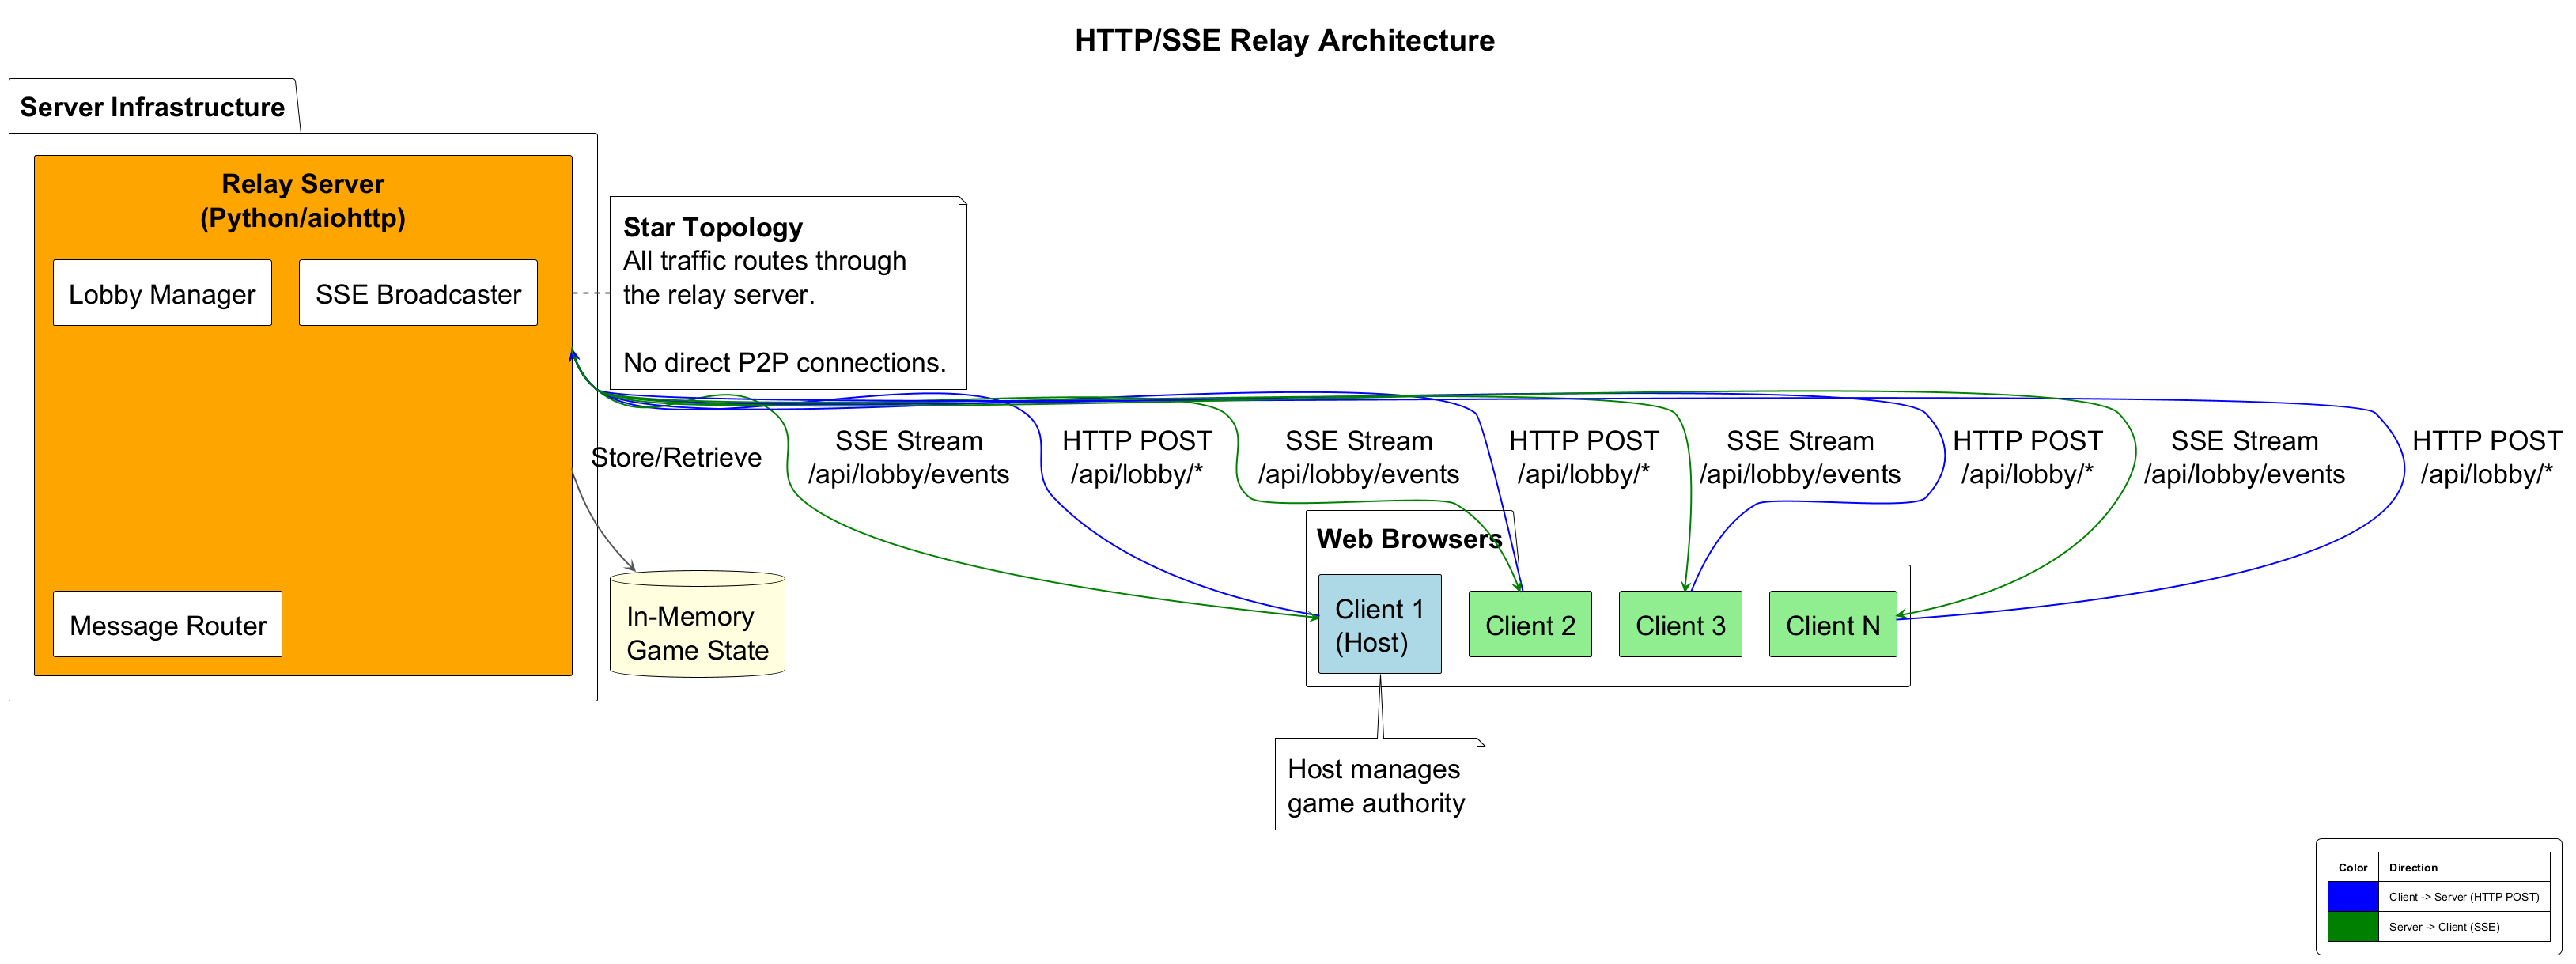
\includegraphics[width=0.82\textwidth]{figures/diagrams/http-sse-architecture.png}
    \caption{HTTP/SSE relay-oriented architecture used for web-first multiplayer synchronization}
    \label{fig:http-sse-architecture}
\end{figure}

%-----------------------------------------------------------------------
\subsection{State Synchronization Patterns}
\label{subsec:state-sync-patterns}

Two synchronization patterns are central:
\begin{itemize}
    \item \textbf{Optimistic local interaction}: local responsiveness is preserved while awaiting authoritative confirmation.
    \item \textbf{Host broadcast reconciliation}: final shared state is re-broadcast to all peers to converge state.
\end{itemize}

\begin{lstlisting}[language=Python, caption={Architectural pattern: host-authoritative move confirmation}]
# Client proposes move -> host validates -> host broadcasts canonical state
on_client_move(card_id, target_slot):
    if host_validate(card_id, target_slot):
        host_apply(card_id, target_slot)
        broadcast_canonical_state(card_id, target_slot)
    else:
        reject_and_restore(card_id)
\end{lstlisting}

This pattern minimizes permanent divergence while preserving interaction fluidity.

%-----------------------------------------------------------------------
\subsection{GDSync Integration Boundary}
\label{subsec:gdsync-integration}

GDSync is treated as a synchronization abstraction layer, while architecture ownership remains in the game managers. This prevented framework-specific behavior from leaking into all gameplay components and reduced replacement cost when debugging framework limitations.
The web-export signaling patch details are intentionally analyzed in Chapter~\ref{ch:problems}, Section~\ref{subsec:web-patch-case-study}, while this section keeps the architectural boundary view.
% TODO: [Artifact] Real (non-pseudocode) manager-boundary code excerpt.
% TODO: [Purpose] Prove the wrapper/delegation boundary and authority checkpoint in actual project code.
% TODO: [Source Inputs] scenes/Multiplayer/MultiplayerGame/multiplayer_card_manager.gd; scenes/Multiplayer/connection_manager.gd.
% TODO: [Placement] Replace the pseudocode listing or place immediately below it.
% TODO: [Done Criteria] Excerpt shows sync entrypoint delegating into manager logic and where authority is enforced.
% TODO: [Cross-refs] Chapter~\ref{ch:problems}, Section~\ref{subsec:web-patch-case-study}.

\begin{lstlisting}[language=Python, caption={Architectural boundary: sync wrapper delegates to game manager}]
@GDSync.rpc(call_local=true)
func sync_move(card_id: int, target_id: int):
    multiplayer_manager.apply_authoritative_move(card_id, target_id)
\end{lstlisting}

%-----------------------------------------------------------------------
\subsection{Connection Management}
\label{subsec:connection-management}

Connection handling is split into phases:
\begin{itemize}
    \item \textbf{Lobby phase}: peer discovery, readiness, and session configuration.
    \item \textbf{Gameplay phase}: synchronized interaction and reconciliation.
    \item \textbf{Failure phase}: disconnection detection and graceful degradation.
\end{itemize}

%-----------------------------------------------------------------------
\section{Data Flow and Visibility Model}
\label{sec:data-flow}

The architecture explicitly distinguishes:
\begin{itemize}
    \item \textbf{Shared-visible state}: container cards and game-level counters.
    \item \textbf{Player-private state}: cards in private buffers hidden from other players.
\end{itemize}

This model is central to the OpenMP analogy: all participants can access shared memory, while local buffer state remains private.
% TODO: [Artifact] Card-move sequence/data-flow diagram.
% TODO: [Purpose] Show end-to-end state transition from user action to converged visibility state.
% TODO: [Source Inputs] scenes/Multiplayer/MultiplayerGame/multiplayer_card_manager.gd; scenes/CardScene/scripts/card_manager.gd.
% TODO: [Placement] Directly after this paragraph and before the visibility listing.
% TODO: [Done Criteria] Must include propose -> validate -> authoritative apply -> broadcast -> visibility-gate update and identify shared vs private divergence points.
% TODO: [Cross-refs] Section~\ref{subsec:state-sync-patterns}; Chapter~\ref{ch:results}, Section~\ref{subsec:learner-messages}.

\begin{lstlisting}[language=Python, caption={Architectural mechanism: private buffer visibility gate}]
if card.in_private_buffer():
    card.visible = (card.buffer_owner_id == local_player_id)
else:
    card.visible = true
\end{lstlisting}

%-----------------------------------------------------------------------
\section{Barrier Synchronization Architecture}
\label{sec:barrier-architecture}

The game includes a barrier synchronization feature that directly models the \texttt{\#pragma omp barrier} construct from OpenMP. Architecturally, the barrier is implemented as a separate \texttt{BarrierManager} component (not embedded in the card manager) following the single-responsibility principle.

\subsection{State Machine Design}
\label{subsec:barrier-state-design}

The barrier operates as a three-state finite automaton with the following transitions:

\begin{enumerate}
    \item \textbf{RUNNING} $\to$ \textbf{WAITING\_AT\_BARRIER}: Any player initiates a barrier; all must arrive.
    \item \textbf{WAITING\_AT\_BARRIER} $\to$ \textbf{BARRIER\_ACTIVE}: All players have reached the barrier; the main thread is granted exclusive access to the shared container.
    \item \textbf{BARRIER\_ACTIVE} $\to$ \textbf{RUNNING}: The main thread releases the barrier; normal play resumes.
\end{enumerate}

This maps directly to OpenMP barrier semantics: threads reaching the barrier must wait until all threads have arrived, after which execution proceeds in a coordinated fashion.

\subsection{Integration Points}
\label{subsec:barrier-integration}

The \texttt{BarrierManager} integrates with the multiplayer card manager through three mechanisms:
\begin{itemize}
    \item \textbf{Signals}: emits \texttt{barrier\_state\_changed} to trigger UI overlays (lock screen for non-main-thread players).
    \item \textbf{GDSync exposure}: barrier functions are registered for remote invocation alongside card synchronization functions.
    \item \textbf{Settings}: BarrierManager reads the barrier mode (first-to-reach or round-robin) from the global \texttt{Settings} autoload.
\end{itemize}

\noindent The barrier implementation details are covered in Chapter~\ref{ch:implementation}, Section~\ref{sec:barrier-implementation}.

%-----------------------------------------------------------------------
\section{Responsive UI/UX Architecture}
\label{sec:responsive-ui-ux}

UI architecture prioritizes interpretable interaction under constrained viewports:
\begin{itemize}
    \item Scrollable container strategy for large card sets.
    \item Buffer-first layout to reinforce shared/private distinction.
    \item Immediate feedback (toast/status indicators) to reduce action ambiguity in multiplayer.
\end{itemize}

%-----------------------------------------------------------------------
\subsection{UI Layering and Overlay Isolation}
\label{subsec:ui-layering}

Overlay and inspection elements are separated from gameplay nodes to minimize accidental coupling between debug/auxiliary UI and gameplay transforms. This layering approach supports live inspection tooling while preserving gameplay interaction consistency.
% TODO: [Artifact] Node-tree snapshot and short explanatory caption for UI layering.
% TODO: [Purpose] Clarify why CanvasLayer-based overlays do not interfere with gameplay-space nodes.
% TODO: [Source Inputs] scenes/MainMenuScene/menu_scene.tscn (CanvasLayer, VarTreeMainMenu).
% TODO: [Placement] In this subsection as a compact figure or annotated listing.
% TODO: [Done Criteria] Clearly shows gameplay nodes vs overlay/debug nodes and the isolation rationale.
% TODO: [Cross-refs] Chapter~\ref{ch:implementation}, Section~\ref{subsec:vartree}.

A playful evasive hover animation is also present in the main menu as a non-critical engagement microinteraction; its reception in early tests is discussed in Chapter~\ref{ch:results}, Section~\ref{subsec:engagement-effects}.

%-----------------------------------------------------------------------
\section{Performance and Scalability Constraints}
\label{sec:performance}

Architecture-level performance strategies include:
\begin{itemize}
    \item bounded synchronization payloads,
    \item authoritative reconciliation instead of full scene replication,
    \item UI/container policies that remain usable at higher card counts.
\end{itemize}

Observed constraints and measured outcomes are discussed in Chapter~\ref{ch:results}.

%-----------------------------------------------------------------------
\section{Summary}
\label{sec:architecture-summary}

This chapter documented architectural decisions that made the tool technically feasible and pedagogically interpretable in a web-first multiplayer context. The focus was on synchronization boundaries, state visibility semantics, and authority patterns rather than exhaustive implementation detail. Detailed implementation evidence is provided in Chapter~\ref{ch:implementation}, while educational and operational effectiveness is evaluated in Chapter~\ref{ch:results}.
